\section{Image (a)}

\begin{wrapfigure}{l}{0.5\textwidth}
    \centering
    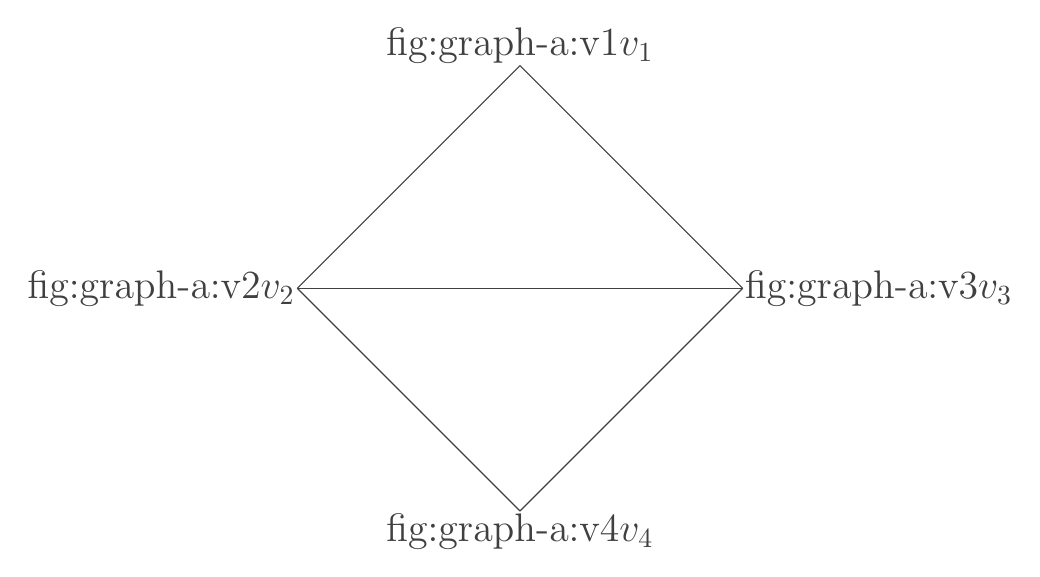
\begin{tikzpicture}[draw=darkgray, text=darkgray, align=center, node distance=4cm]
    \tikzstyle{every node}=[inner sep=0pt];

    \node (v1) [label=above:{\Large\hypertarget{fig:graph-a:v1}{$v_1$}}] {};
    \node (v2) [label=left:{\Large\hypertarget{fig:graph-a:v2}{$v_2$}}, below left of = v1] {};
    \node (v3) [label=right:{\Large\hypertarget{fig:graph-a:v3}{$v_3$}}, below right of = v1] {};
    \node (v4) [label=below:{\Large\hypertarget{fig:graph-a:v4}{$v_4$}}, below right of = v2] {};

    \path (v1.center)
        edge (v2.center)
        edge (v3.center);
    \path (v4.center)
        edge (v2.center)
        edge (v3.center);
    \path (v2.center)
        edge (v3.center);
\end{tikzpicture}


    \caption{Image \texttt{a.} from question with labelled nodes.}
    \label{fig:graph-a}
\end{wrapfigure}

A \textbf{trail} is a sequence of \textit{distinct} edges such that any consecutive edges are incident to a common vertex. When the sequence visits every edge of a graph, it is called an \textbf{Euler trail}. Following such trail with a pencil would lead us to draw the graph with the specified requirements.

To find if a graph has an Euler trail, however, we need \nameref{thm:euler-circuit}, which is stated in terms of a \textbf{circuit}, that is, a trail that ends at the same vertex it started. From there we have \cref{thm:euler-trail}, which won't be proved here, but the main argument behind it is:

If we connect the two vertices with odd degree by an edge $e := x y$, we get an even graph. Since this new graph has an Euler circuit $W := u W_1 x e y W_2 u$ and the only edge missing is $e$, the trail $T := x W_1 u W_2 y$ still is eulerian for the original graph.

~

\begin{theorem}[Euler's Theorem] \label{thm:euler-circuit}
    A connected graph has an Euler circuit if and only if every vertex has even degree.
\end{theorem}

\begin{proposition} \label{thm:euler-trail}
    A connected graph has an Euler trail if and only if exactly zero or two vertices have odd degree.
\end{proposition}

\subsection{Answer} \label{sec:graph-a}

    Finally, by \cref{thm:euler-trail}, we can see that the graph in \cref{fig:graph-a} can be drawn without raising the pencil and without repeating any lines. This is because only $\hyperlink{fig:graph-a:v2}{v_2}$ and $\hyperlink{fig:graph-a:v3}{v_3}$ have odd degree ($\deg(\hyperlink{fig:graph-a:v2}{v_2}) = 3 = \deg(\hyperlink{fig:graph-a:v3}{v_3})$).

    Furthermore, considering the argument for \cref{thm:euler-trail}, we must start the drawing at one of the two odd vertices, $\hyperlink{fig:graph-a:v2}{v_2}$ or $\hyperlink{fig:graph-a:v3}{v_3}$.
